\section{Datasets}

Labeled data has a crucial influence on algorithm development and evaluation in
research fields dealing with classification and detection. Any machine learning algorithm is only as good as the data behind it in terms of modeling and generalization
properties.

Well-established and easily accessible benchmark databases attract the interest of the research community as readily available support for research, thus accelerating the pace of development for related fields. There are many well-known databases in related research areas, such as TIMIT \cite{garofolo1993darpa} for speech
recognition or the Million Song Dataset \cite{bertin2011million} for various tasks in music information retrieval. In view of this critical influence, the process of creating
a dataset for system developing is, naturally, very delicate. The content must be carefully selected to provide sufficient coverage of the aspects of interest, sufficient variability in characterizing these aspects, and a sufficient quantity of examples for robust modeling. Unfortunately, there is no rule on what ``sufficient'' means, as it usually depends on the projected use of the data.


Compared to speech, the categories and sequences of sound events are not so straightforward to define, as any object or being may produce a sound. Sounds can be organized into categories based on different properties, such as the sound source (e.g., cup), its production mechanism (e.g., hit), or even the source properties (e.g., metal), and the same sound can belong to many different categories, depending on the chosen property (sound when hitting a metallic cup). In addition, there are no specific rules on how environmental sounds co-occur. 

For this reason, building a database for environmental sounds
is a complicated task, with the choice of classes usually dictated by the targeted
research, and the size limited by practical aspects of data collection especially compared to well-known datasets available for image processing (i.e., Imagenet\cite{deng2009imagenet}). Anyway, very recently a project promoted by Google has been presented \cite{gemmeke2017audio}, with the aim to collect a large human annotated dataset and a relative ontology obtained from YouTube videos.

\subsection{Dataset Acquisition}

Recording real-world audio is the obvious data collection method for obtaining
realistic data. Creating a new dataset by recording new data has the advantage of
producing a collection with controlled audio quality and content.

Typically, the recording settings such as microphone type, number of channels, sample rate, bit depth are defined in the planning phase of the project, and often they also depend on the final objectives of the project (i.e., a mobile application vs. a research corpus). Anyway, the most common sampling settings are 44.1 kHz, 16 bit respectively for sampling-rate and bit depth. Numerous computational auditory scene analysis research projects make use of binaural heads setups (\figref{fig:binaural}), with the aim to replicate the frequency-dependent distortions of phase and amplitude on sounds produced by the human auditory system.

\begin{figure}[h]
	\centering
	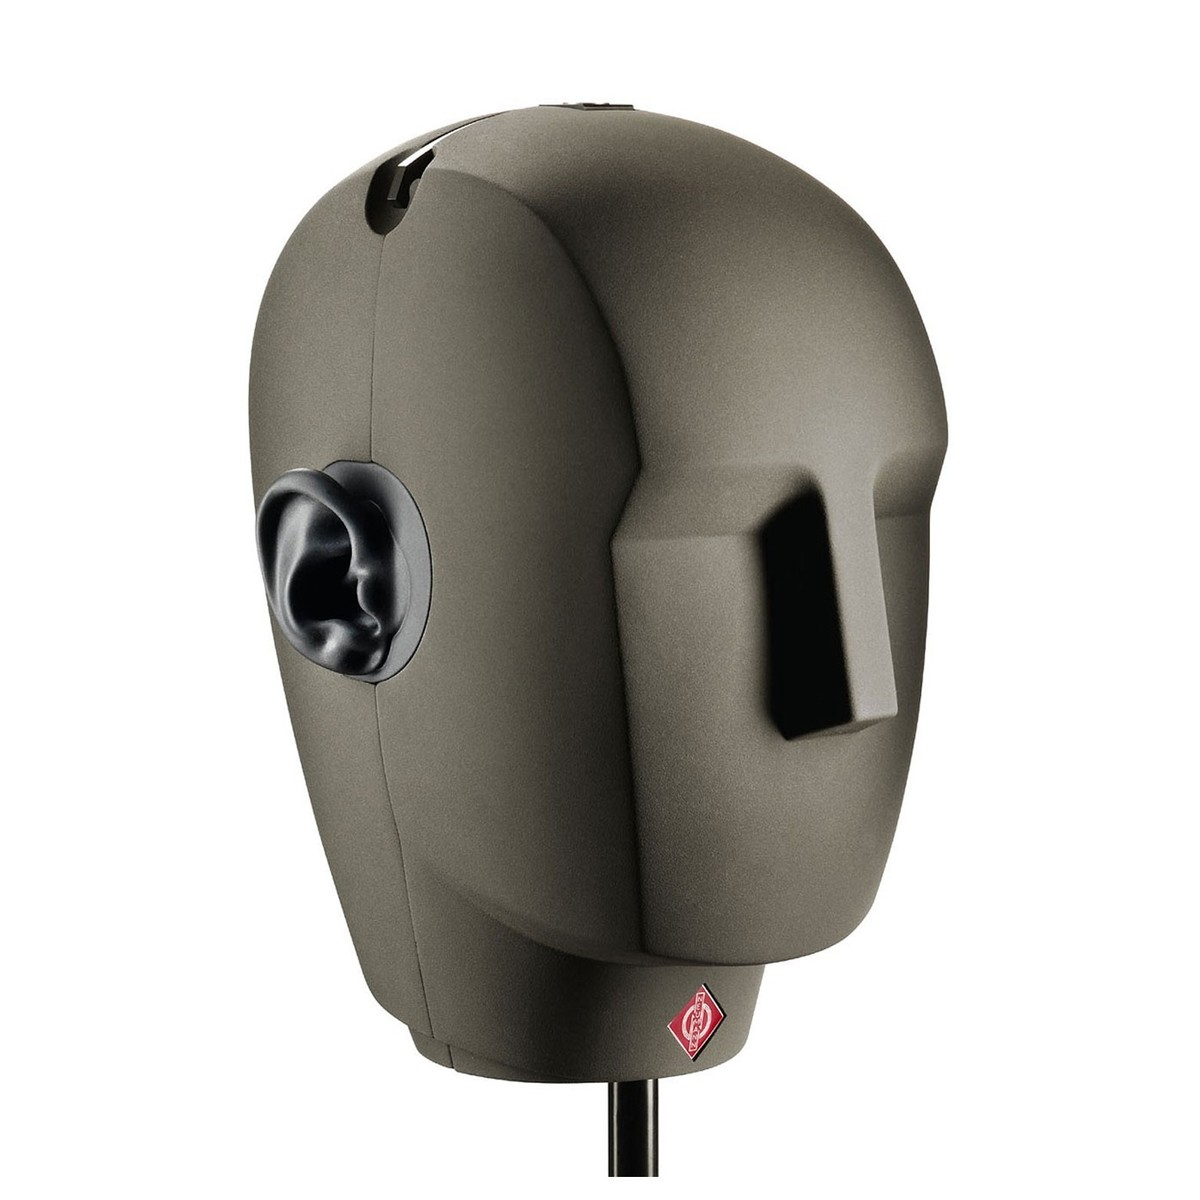
\includegraphics[width=0.5\textwidth]{img/binaural.jpg}
	\caption[Dummy head]{Dummy head for binaural recording.}
	\label{fig:binaural}
\end{figure}

Although the use
of the same settings and device(s) throughout the data will result in a better
quality set, some recent algorithms are designed to counteract these diversities, leading to the possibility to gather material from different recording campaigns. 
In fact, one disadvantage of recording new data is that in order to cover as much acoustic variability
and diversity as possible, recordings must be done in many different conditions.
For location-specific modeling, this may mean different weather or human activity
conditions, while for more general modeling, it would also require traveling to
other locations, adding significant time and effort to the data collection procedure.

\subsection{Dataset Labelling}
Labeled data has a crucial influence on algorithm development and evaluation in
research fields dealing with classification and detection. The textual labels used
in annotation must provide a good description of the associated category and not
allow misinterpretation. To allow supervised learning and evaluation, the audio must have corresponding
reference annotations. These annotations can be produced manually or in various
semi-automatic ways, with the quality and level of detail available in the obtained
annotation often depending on the procedure used. Manual annotation involves
human annotators that will produce a mapping of the audio content into textual
labels. Manually annotating sound scene audio material is relatively fast, while for
sound events the process is much slower, with annotation using weak labels being
much faster than with strong labels. Manual annotation is prone to subjectivity
arising from the selection of words for labels and placing of temporal boundaries.

\subsection{Acoustic Features}
\label{ssec:ac_features}
The time domain representation of a sound signal, or waveform, is not easy to
interpret directly. Therefore, frequency-domain representations and time-frequency domain

representations (including multiscale representations) have been used for years
providing \textit{features} of the sound signals that are more in line with the human
perception. In this section we report a brief description of the most commons.

\subsubsection{Mel Frequency Cepstral Coefficients}
MFCCs is a well-known set of features widely employed in audio applications, especially for the purpose of representing speech data. Indeed, the weighting operation performed by the Mel bands emulates the frequency response of
the human hearing organ, which is sensible at its most to speech frequencies.
The extraction procedure requires few stages. An excerpt of the signal is
 transformed in the frequency domain by means of STFT. The obtained spectrum is hence mapped to the mel scale by using triangular overlapping windows.
For each mel frequency the logs of the powers are considered, to whom the Discrete Cosine Transform (DCT) is applied. The resulting spectrum are the

MFCCs. Furthermore, a common procedure consists in concatenating MFCCs
with their first and second derivatives, in order to provide a temporal evolution
of the signal.

\subsubsection{LogMel}

LogMel features have been recently applied in the field of acoustic modelling
and music structure analysis [57, 58], leading to encouraging results. The procedure for LogMel extraction shares several aspects with the one described
for MFCCs features. In details, a set of mel-band filters is applied to the
spectrogram of the signal, from which the logarithm of the power spectrum
for each band is considered. The logarithmic transformation is applied to each sub-band energy in order to match the human perception of loudness.
However, due to the absence of the DCT, no
spatial compression is performed to the features, which remain correlated in
the frequency domain. In this work, the employment of LogMel matches the
choice of using some of the systems proposed in the next chapters (e.g., CNNs),
where the objective is to exploit the intrinsic correlation of input features in

order to highlight repetitive patterns present in the features.

\subsubsection{Pitch}
The tone of human voice is highly characteristic, for that reason is used i.e. in VAD systems. The Sub-Harmonic-Summation (SHS) method described in \cite{hermes1988measurement} is one of the most common algorithms. In particular, the spectrum is shifted along the log-frequency axis, for each shift the spectrum is scaled and then summed. This procedure creates the sub-harmonic summation spectrum, where peak picking is applied to determine pitch. The used frame size is equal to 50\,ms.


\subsubsection{WC-LPE Feature}
The Wavelet Coefficient (WC) and Linear Prediction Error (LPE) feature set has been recently developed and exploited for audio onset detection purpose \cite{marchi2014multi}. WC-LPE carries information on non-stationary parts of the signal, thus, it can facilitate the speech boundaries identification.
Firstly, the signal undergoes the Discrete Wavelet Transformation (DWT). Then, each sub-band of the wavelet-domain is filtered by a set of Linear Prediction Error Filter (LPEFs) and Forward Prediction Errors (FPE) are extracted. Finally, the first derivatives are obtained from wavelet coefficients and added to them in order to form the feature set.


\subsubsection{RASTA-PLP}
With RASTA-PLP we refer to RelAtive SpecTrAl transform - Perceptual Linear Prediction, a feature set often exploited to represent speech \cite{hermansky1994rasta}.
Short-term noise variations are smoothed and the constant offset is removed by RASTA filtering procedure, while the task of PLP is to simulate several well-known properties of the hearing system.

\subsubsection{Scattering Transform}

The scattering transform \cite{Mallat2012} is the operation on which the Deep Scattering Spectrum (SCAT) is based. SCAT is a multi-resolution representation of a signal based on a tree of complex wavelet filters followed by a non-linearity. SCAT proves successful in gathering information at multiple resolutions on non-stationary signals thanks to its good properties, such as translation invariance, stability to small diffeomorphisms and uniqueness, e.g., time-warping deformations.


\subsection{Data Augmentation}
Data augmentation refers to methods for increasing the amount of development data
available without additional recordings. With only a small amount of data, systems
often end up overfitting the training data and performing poorly on unseen data.
Thus, it is desirable to artificially increase the amount and diversity of data used in
training. 

Many techniques have been proposed for data augmentation in domains different from audio. In the case of image processing, affine transformations such as rotation, shear, scaling or zooming are very common perturbations to apply directly on the raw data (i.e., the images composing the dataset) in order to augment the training sets of the systems. Some approaches extend the augmentation in the feature space \cite{li2014learning}.
Dataset augmentation could be used to reduce overfitting while training supervised learning models or to counteract the dataset imbalance i.e., if the classes are not approximately equally represented as in the case of SMOTE \cite{chawla2002smote, han2005borderline}. 

In the audio field, data augmentation exploits techniques such as pitch shifting, time stretching or the generation of multi-microphone data by means of simulated impulse response of the acoustic space or performing the transformation not in input space, but in the feature space. Adding random gaussian noise to the input data (raw waveform or acoustic features) can also be seen as a data augmentation technique for the audio domain.

With the development of the artificial neural networks (ANN), some works act this augmentation by means of auto-encoder model also using Generative ANN. The above mentioned approaches have a large impact in the development of data driven approaches to activity recognition, with applications in the Active and Assisted Living (AAL) domain that has a lack of large scale, high quality, and annotated datasets even if open datasets are growing. In particular, these models are trained to reproduce the signal they have been trained with, and if their latent space is properly perturbed, they are able to generate new data, useful to extend the training sets of detection/classification systems. In this context we can also mention the Generative Adversarial Networks (GAN) (cf. \secref{ssec:GAN}). 

A limited number of repositories have supported the notion of shared datasets, including a small number of activity recognition related resources. To address this lack it is possible to simulate smart environments equipped with heterogeneous sensors and combine the signals from different domains with novel data augmentation techniques exploiting the aforementioned deep learning techniques.

\newpage
\section{Evaluation Setup}
During system development, iterative training and testing of the system is necessary
for tuning its parameters. For this purpose, the labeled data available for development is split into disjoint training and testing sets. However, labeled data is often in short supply, and it is difficult to choose between using more data for training (leading to better-performing systems) or for testing (giving more precise and
reliable estimates of system performance). For an efficient use of all the available
data, system development can use cross-validation folds to artificially
create multiple training/testing splits using the same data; overall performance is
then the average of performance on each split. Cross-validation folds also help avoid
overfitting and supports generalization properties of the system, so that when the
system is used on new data it is expected to have similar performance as seen with
the data used for development.

As shown in \figref{fig:cross-valid}, one round of cross-validation involves partitioning a sample of data into complementary subsets, performing the analysis on one subset (called the training set), and validating the analysis on the other subset (called the validation set or testing set). To reduce variability, multiple rounds of cross-validation are performed using different partitions, and the validation results are then combined over the rounds to give an estimate of the model’s predictive performance. 


Cross-validation folds also help avoid overfitting and supports generalization properties of the system, so that when the
system is used on new data it is expected to have similar performance as seen with the data used for development.

If available, a separate set of examples with reference annotation can be used to evaluate the generalization properties of the fully tuned system. We refer to this set as \textit{evaluation set}, and use it to evaluate how the system would perform on new data.

\begin{figure}[h]
	\centering
	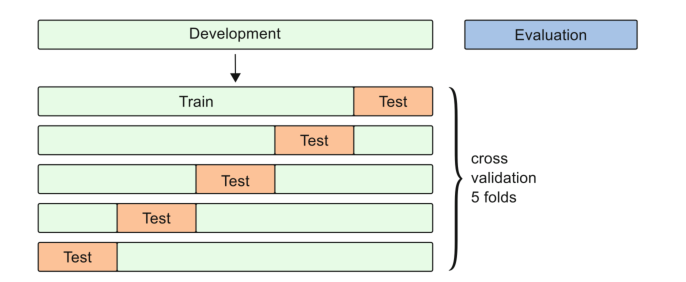
\includegraphics[width=0.8\textwidth]{img/cross-valid}
	\caption[Cross-Validation Splitting]{Splitting a dataset into development and evaluation data, with five folds for crossvalidation during system development. Picture courtesy of \cite{virtanen2018computational}.}
	\label{fig:cross-valid}
\end{figure}

\newpage
